\chapter{Measurement in Science: Units and Instruments}\label{ch:g6:measurement-in-science}

A carpenter, a doctor and an astronomer walk into their workdays:
one \omterm{def:g6:measurement-in-science:measuring}{measures} a shelf, one a fever, one the wanderings of Mars. All
three trust the same quiet machinery --- agreed \omterm{def:g6:measurement-in-science:measuring}{units}, honest
instruments, careful reading. This year physics turns properly
quantitative, so we begin by polishing the tools every later
chapter will lean on.

\section{From seeming to number}

Five years of experiments have taught us a rhythm: eyes and hands
guess, instruments decide. Ruler against seeming-longer; balance
against seeming-heavier; \omterm{def:g3:temperature-thermometers:temperature}{thermometer} against feeling-cold. Each
time, the instrument's verdict is a \emph{number with a \omterm{def:g6:measurement-in-science:measuring}{unit}} ---
and that pair travels, compares, and can be checked by anyone,
which no feeling ever could.

\begin{definition}[Measuring a quantity]\label{def:g6:measurement-in-science:measuring}
To \emph{measure}\index{measure} a quantity --- a length, a \omterm{def:g3:measuring-mass:mass}{mass}, a
\omterm{def:g2:measuring-time:duration}{duration}, a \omterm{def:g3:temperature-thermometers:temperature}{temperature} --- is to count how many times its agreed
\emph{unit}\index{unit} fits into it, using an instrument built for
the job. The result is always written as a number \emph{with} its
unit: \qty{28.5}{cm}, \qty{450}{g}, \qty{37.2}{\celsius}. A number
alone is a rumor; number-plus-unit is a measurement.
\end{definition}

\begin{example}[The price of a missing unit]\label{ex:g6:measurement-in-science:missing}
``Add 3 of flour.'' \omterm{def:g3:measuring-mass:units}{Grams}? Spoonfuls? Cups? The cake's fate hangs
on the missing word. Real disasters have followed missing or
mixed-up \omterm{def:g6:measurement-in-science:measuring}{units} --- pilots have run out of fuel mid-flight because
\omterm{def:g3:measuring-mass:units}{kilograms} were confused with pounds. Professionals write the \omterm{def:g6:measurement-in-science:measuring}{unit}
every time, without exception; from this chapter on, so do we.
\end{example}

\section{The world's units}

\begin{definition}[The scientist's starter kit]\label{def:g6:measurement-in-science:units}
The world has agreed on common \omterm{def:g6:measurement-in-science:measuring}{units}, one family per quantity:
\begin{enumerate}
  \item length: the \emph{\omterm{def:g2:measuring-length:units}{metre}} (\unit{m}), with its offspring
        the kilometre ($\qty{1}{km} = \qty{1000}{m}$), \omterm{def:g2:measuring-length:units}{centimetre}
        ($\qty{100}{cm} = \qty{1}{m}$) and millimetre
        ($\qty{1000}{mm} = \qty{1}{m}$);
  \item \omterm{def:g3:measuring-mass:mass}{mass}: the \emph{\omterm{def:g3:measuring-mass:units}{kilogram}} (\unit{kg}), with the \omterm{def:g3:measuring-mass:units}{gram}
        ($\qty{1}{kg} = \qty{1000}{g}$) and milligram
        ($\qty{1000}{mg} = \qty{1}{g}$);
  \item time: the \emph{second} (\unit{s}), with the minute
        ($\qty{1}{min} = \qty{60}{s}$) and hour
        ($\qty{1}{h} = \qty{60}{min} = \qty{3600}{s}$);
  \item \omterm{def:g3:temperature-thermometers:temperature}{temperature}: the \omterm{def:g3:temperature-thermometers:temperature}{degree Celsius} (\unit{\celsius});
  \item volume of \omterm{def:g3:solids-liquids-gases:liquid}{liquids}: the litre (\unit{L}), which we \omterm{def:g6:measurement-in-science:measuring}{measure}
        out in the next chapter.
\end{enumerate}
\end{definition}

\begin{example}[Converting like a scientist]\label{ex:g6:measurement-in-science:convert}
Conversions are rides on the decimal staircase.
$\qty{2.35}{m}$ in \omterm{def:g2:measuring-length:units}{centimetres}: multiply by $100$ --- the point
slides two places right: \qty{235}{cm}. $\qty{4500}{g}$ in
\omterm{def:g3:measuring-mass:units}{kilograms}: divide by $1000$: \qty{4.5}{kg}. Time is the rebel of
the family --- its steps are $60$, not $10$: $\qty{2.5}{min}$ is
not $250$ seconds but $2 \times 60 + 30 = \qty{150}{s}$. Respect
the rebel.
\end{example}

\begin{remark}[Who guards the metre?]\label{rem:g6:measurement-in-science:guard}
For two centuries, the world's \omterm{def:g2:measuring-length:units}{metre} was a bar of precious metal
in a guarded vault near a great European capital, and the \omterm{def:g3:measuring-mass:units}{kilogram}
a gleaming cylinder beside it: every nation's rulers and \omterm{def:g4:weight-and-mass:weight}{weights}
were copies of copies of those. Today the guards have been
retired: the \omterm{def:g2:measuring-length:units}{metre} and its friends are now defined from
unchangeable facts of nature itself --- \omterm{def:g1:light-and-shadows:source}{light} and the inner clocks
of atoms --- so that any well-equipped laboratory on Earth (or
beyond it!) can rebuild them exactly. \omterm{def:g6:measurement-in-science:measuring}{Units} are humankind's
longest-running peaceful agreement.
\end{remark}

\begin{omfigure}
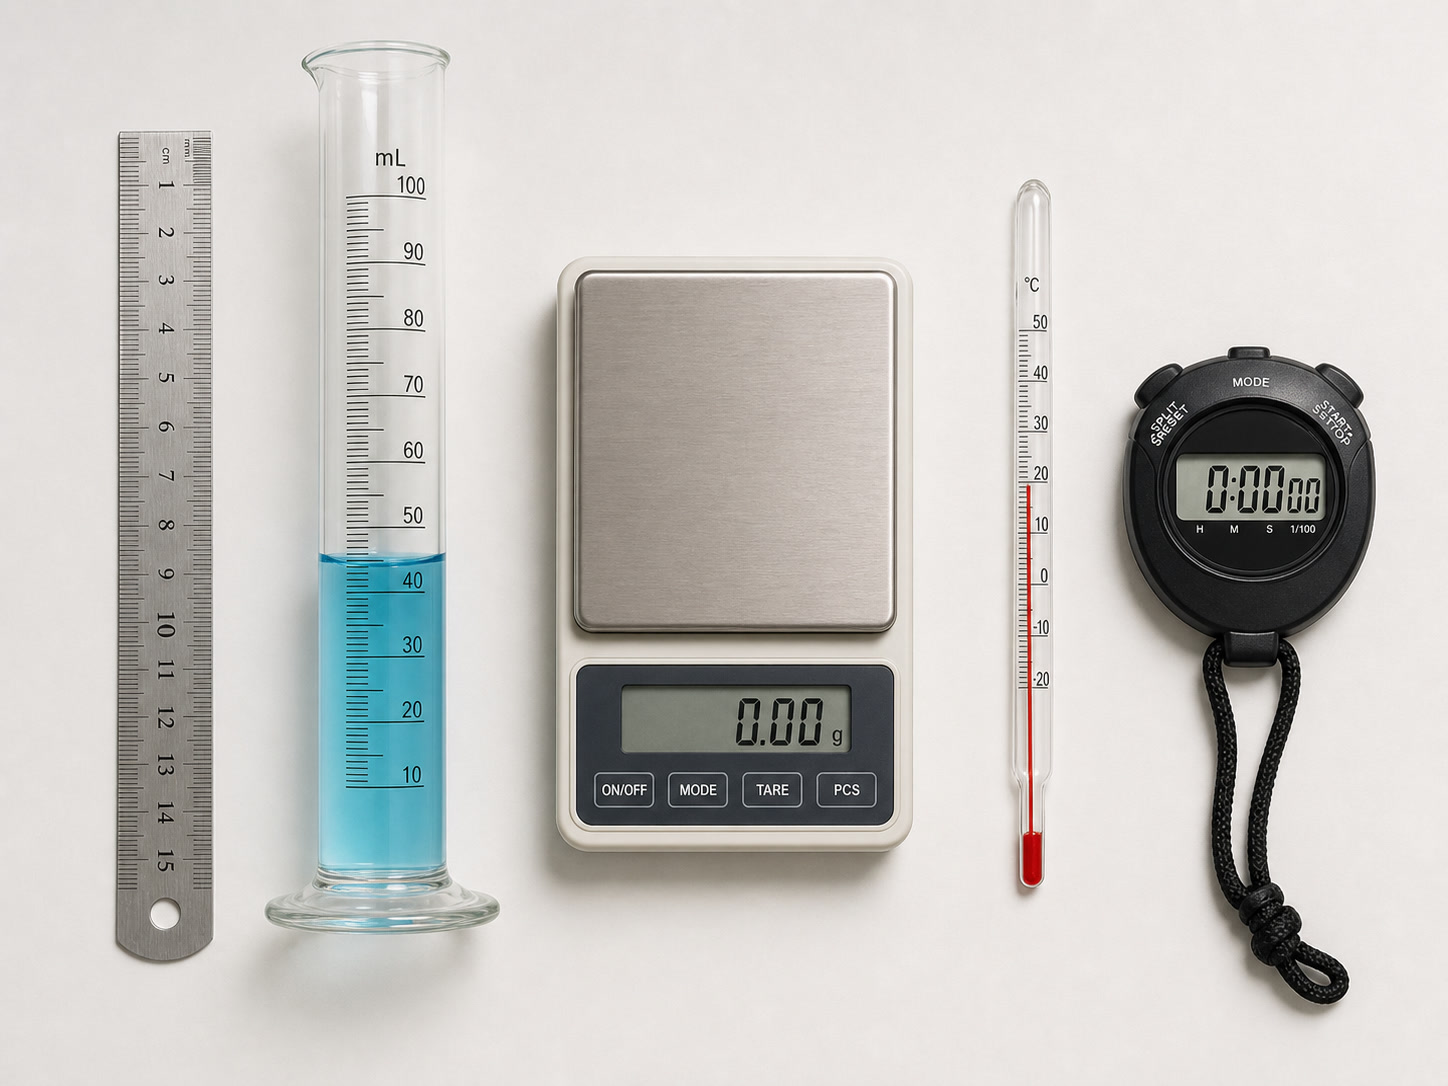
\includegraphics[width=0.55\linewidth]{images/book1/ai/g6-measurement-instruments.jpg}

{\small The measurer's toolkit: length, volume, \omterm{def:g3:measuring-mass:mass}{mass}, \omterm{def:g3:temperature-thermometers:temperature}{temperature} and time, each with its own instrument and its own \omterm{def:g6:measurement-in-science:measuring}{unit}.}
\end{omfigure}

\section{Using instruments well}

\begin{method}[Reading any graduated scale]\label{met:g6:measurement-in-science:read}
Rulers, \omterm{def:g3:temperature-thermometers:temperature}{thermometers}, measuring jugs, dials: one skill reads them
all.
\begin{enumerate}
  \item find the \emph{graduation value}: pick two neighboring
        numbered marks, subtract, and divide by the number of
        little steps between them --- on a ruler numbered every
        \omterm{def:g2:measuring-length:units}{centimetre} with ten steps, each step is
        $1 \div 10 = \qty{0.1}{cm}$, one millimetre;
  \item put your eye squarely in front of the mark (a slanted view
        shifts the reading);
  \item count on from the last numbered mark: $7$ and $3$ little
        steps is $7.3$;
  \item write the number \emph{with its \omterm{def:g6:measurement-in-science:measuring}{unit}}.
\end{enumerate}
\end{method}

\begin{omfigure}
\begin{tikzpicture}[scale=0.85]
  \draw[thick] (0.4,0.6) -- (10.8,0.6);
  \foreach \x/\l in {0.8/5, 3.0/6, 5.2/7, 7.4/8, 9.6/9} {
    \draw[thick] (\x,0.6) -- (\x,1.35);
    \node[above, font=\small] at (\x,1.4) {\l};
  }
  \foreach \i in {1,...,9} {
    \draw (0.8+\i*0.22,0.6) -- (0.8+\i*0.22,1.0);
    \draw (3.0+\i*0.22,0.6) -- (3.0+\i*0.22,1.0);
    \draw (5.2+\i*0.22,0.6) -- (5.2+\i*0.22,1.0);
    \draw (7.4+\i*0.22,0.6) -- (7.4+\i*0.22,1.0);
  }
  \draw[-Stealth, very thick, omThm] (5.86,2.1) -- (5.86,1.15);
  \node[above, font=\small, omThm] at (5.86,2.15)
    {here: $7$ and $3$ steps $= 7.3$};
  \node[below, font=\small] at (5.6,0.3)
    {ten steps per unit, so each step is worth $0.1$};
\end{tikzpicture}

{\small Reading a graduated scale: first learn what one little step
is worth, then count on from the last numbered mark.}
\end{omfigure}

\begin{method}[Estimate, measure, judge]\label{met:g6:measurement-in-science:estimate}
Professionals never \omterm{def:g6:measurement-in-science:measuring}{measure} cold:
\begin{enumerate}
  \item \emph{estimate} first --- ``this table is about two
        \omterm{def:g2:measuring-length:units}{metres}'';
  \item \emph{choose} the instrument whose range and steps fit the
        job (a ruler for a stamp, a tape for a corridor, kitchen
        scale for flour, bathroom scale for people);
  \item \emph{\omterm{def:g6:measurement-in-science:measuring}{measure}}, by the reading rules;
  \item \emph{judge}: does the result agree roughly with the
        estimate? A table measured at \qty{21.3}{m} did not grow
        --- you misread by a factor of ten, and the estimate just
        caught it.
\end{enumerate}
The estimate is your safety net: it catches slipped decimal points
before they catch you.
\end{method}

\begin{example}[Choosing wisely]\label{ex:g6:measurement-in-science:choose}
To weigh a letter for posting, the bathroom scale is useless ---
the letter's \qty{18}{g} vanish between its steps; the kitchen
scale, stepping by the \omterm{def:g3:measuring-mass:units}{gram}, answers perfectly. To time a
$100$-metre sprint, the kitchen clock's minute steps are hopeless;
a stopwatch counts in hundredths of a second. Neither instrument
is ``better'': each has a territory, set by its range and its
smallest step.
\end{example}

\section{Honest numbers}

\begin{remark}[Between the marks]\label{rem:g6:measurement-in-science:between}
Real needles love to land between marks. Honesty then has two
levels: at least, name the two neighbors --- ``between $7.3$ and
$7.4$, closer to $7.3$''; better, estimate one digit beyond the
marks --- ``about \qty{7.32}{cm}''. What honesty forbids is
inventing precision: reading \qty{7.3214}{cm} off millimetre marks
is fiction wearing a lab coat. An instrument's marks set the limit
of what it can promise.
\end{remark}

\begin{example}[Measure twice, trust more]\label{ex:g6:measurement-in-science:repeat}
Three friends time the same toy car run with the same stopwatch:
\qty{4.6}{s}, \qty{4.8}{s}, \qty{4.7}{s}. Nobody blundered ---
fingers simply start and stop a hair apart. Small scatter is the
normal breath of real measurement. The wise habits: repeat the
measurement, watch the readings huddle, and distrust any single
lonely number --- especially your own.
\end{example}

\section{Exercises}

\begin{exercise}[$\star$]\label{exo:g6:measurement-in-science:1}
Complete each measurement with a sensible \omterm{def:g6:measurement-in-science:measuring}{unit}: a door is $2$
\dots\ tall; \ a coin has \omterm{def:g3:measuring-mass:mass}{mass} $8$ \dots; \ a school lesson lasts
$55$ \dots; \ a fever is $39$ \dots
\end{exercise}

\begin{exercise}[$\star$]\label{exo:g6:measurement-in-science:2}
Convert: \qty{3.2}{m} to \unit{cm}; \ \qty{750}{g} to \unit{kg}; \
\qty{4}{min} to seconds; \ \qty{5600}{m} to \unit{km}.
\end{exercise}

\begin{exercise}[$\star$]\label{exo:g6:measurement-in-science:3}
Why is time the rebel of the \omterm{def:g6:measurement-in-science:measuring}{unit} family? Convert \qty{3.5}{min}
to seconds --- and say what wrong answer the decimal staircase
would have given.
\end{exercise}

\begin{exercise}[$\star$]\label{exo:g6:measurement-in-science:4}
A jug is numbered every \qty{100}{mL} with five little steps
between numbers. What is one step worth? The juice stands two
steps above the $300$ mark --- how much juice?
\end{exercise}

\begin{exercise}[$\star$]\label{exo:g6:measurement-in-science:5}
Which instrument for each job, and why: weighing a pinch of
yeast; \ timing a heartbeat count; \ the width of this page; \ the
length of the schoolyard?
\end{exercise}

\begin{exercise}[$\star$]\label{exo:g6:measurement-in-science:6}
Nadia \omterm{def:g6:measurement-in-science:measuring}{measures} her pencil: \qty{17.4}{m}. Which safety net of
\cref{met:g6:measurement-in-science:estimate} should have caught
this, and what is the likely true value?
\end{exercise}

\begin{exercise}[$\star$]\label{exo:g6:measurement-in-science:7}
A \omterm{def:g3:temperature-thermometers:temperature}{thermometer}'s column stops between the $18$ and $19$ marks,
nearer $19$. Give one honest way to report it --- and one
dishonest report to avoid.
\end{exercise}

\begin{exercise}[$\star$]\label{exo:g6:measurement-in-science:8}
Three stopwatch readings of one run: \qty{6.1}{s}, \qty{6.3}{s},
\qty{6.2}{s}. Is someone at fault? What is the wise report?
\end{exercise}

\begin{exercise}[$\star\star$]\label{exo:g6:measurement-in-science:9}
A recipe abroad asks for ``a quarter pound of butter''. Your
kitchen scale speaks \omterm{def:g3:measuring-mass:units}{grams}, and a full pound is about
\qty{450}{g}. How many \omterm{def:g3:measuring-mass:units}{grams} do you weigh out? What does this
errand teach about shared \omterm{def:g6:measurement-in-science:measuring}{units}?
\end{exercise}

\begin{exercise}[$\star\star$]\label{exo:g6:measurement-in-science:10}
A ruler's first \omterm{def:g2:measuring-length:units}{centimetre} is worn away, so its edge starts at the
$1$ mark. A stamp laid from the edge reads $3.4$ at its far end.
How wide is the stamp really? What habit defeats worn rulers?
\end{exercise}

\begin{exercise}[$\star\star$]\label{exo:g6:measurement-in-science:11}
The class \omterm{def:g6:measurement-in-science:measuring}{measures} the corridor with a \qty{20}{m} tape twice:
\qty{18.25}{m} and \qty{18.35}{m}. The teacher writes
``\qty{18.3}{m}''. Explain her choice, using
\cref{rem:g6:measurement-in-science:between} and
\cref{ex:g6:measurement-in-science:repeat}.
\end{exercise}

\begin{exercise}[$\star\star\star$]\label{exo:g6:measurement-in-science:12}
An old tale: a king decreed his own foot the kingdom's \omterm{def:g6:measurement-in-science:measuring}{unit} of
length. List two practical disasters that follow (think of
carpenters in distant towns, and of the king's growing son as
heir), and explain how the retired metal bar of
\cref{rem:g6:measurement-in-science:guard} solved both --- and
what problem even the bar left unsolved that nature's own
constants finally fixed.
\end{exercise}

\section{Problem: The Instrument Inspector}

\begin{problem}[{Weekend problem --- a day with the town's
instrument inspector; scales, jugs and clocks on trial; the
apprentice's notebook}]\label{pb:g6:measurement-in-science:1}
Every year the town's inspector tests the instruments of shops and
schools. Today you are the apprentice, notebook in hand.

\medskip\noindent\textbf{Part I --- The bakery's scale.}
The inspector carries certified blocks: \qty{500}{g},
\qty{200}{g}, \qty{200}{g}, \qty{100}{g}, \qty{50}{g}.
\begin{enumerate}
  \item She checks that the empty scale's needle stands exactly on
        zero. Why must this be the first test of all?
  \item She loads the \qty{500}{g} and one \qty{200}{g} block. What
        should an honest scale read?
  \item The needle shows \qty{680}{g} instead. Does this scale
        flatter the baker or the customers? Explain who loses
        money on every sale.
  \item Which combinations of her blocks let her test the reading
        \qty{750}{g}? Give one.
  \item The bakery's scale steps by \qty{5}{g}. Could the
        inspector use it to check a \qty{2}{g} letter stamp?
        Why not?
\end{enumerate}

\medskip\noindent\textbf{Part II --- The school's measuring jugs.}
\begin{enumerate}[resume]
  \item A jug is numbered every \qty{200}{mL}, with four steps
        between numbers. What is each step worth?
  \item Water stands one step above the \qty{600}{mL} mark. The
        teacher's log says ``about \qty{700}{mL}''. Grade that
        report: honest, too vague, or fiction?
  \item A pupil reads the jug from a low chair, eye well below the
        water line, and gets a different number than the
        inspector. Which reading rule was broken?
  \item The inspector pours the jug's declared \qty{650}{mL} into
        a certified jug, which shows \qty{640}{mL}. By how much is
        the school jug off, and is that worse or better than one
        of its own steps?
\end{enumerate}

\medskip\noindent\textbf{Part III --- Clocks, and the apprentice's
verdict.}
\begin{enumerate}[resume]
  \item The station clock is checked against the radio time
        signal: it shows the signal's noon at $12$ h $2$ min. Fast
        or slow, and by how much?
  \item If nobody corrects it, how far ahead will it be after a
        week? (It gains the same each day.)
  \item Three shops' clocks show $12$ h $2$ min, $11$ h $58$ min,
        and $12$ h exactly at the signal's noon. The inspector
        says: ``Averaging would be silly here --- fix each
        clock.'' What repair does each need?
  \item Evening. In your notebook, write the inspector's three
        golden rules --- one about zero, one about reading, one
        about \omterm{def:g6:measurement-in-science:measuring}{units} --- each in a single sentence of your own.
\end{enumerate}
\end{problem}
